\uuid{VLwo}
\titre{Reconnaître une bande du plan}
\niveau{L3}
\module{OPTRN}
\chapitre{Réseaux de neurones}
\sousChapitre{Classification}
\theme{Perceptrons, intersection de demi-plans}
\auteur{Maxime Nguyen}
\datecreate{2026-09-26}
\organisation{AMSCC}
\difficulte{2}

\contenu{
\texte{Un point $(x,y)$ reçoit l'étiquette $1$ si les deux mesures $x$ et $y$ diffèrent d'au plus une unité :
\[
B=\{(x,y)\in\mathbb{R}^2\mid |x-y|\leq1\}.
\]
Il reçoit l'étiquette $0$ sinon. On pose $H(t)=1$ si $t\geq0$ et $H(t)=0$ si $t<0$.}

\begin{enumerate}
\item \question{Représenter $B$ dans le plan et traduire la condition $|x-y|\leq1$ par deux inégalités affines.}
\indication{Écrire $-1\leq x-y\leq1$.}
\reponse{$B$ est la bande fermée comprise entre les droites $y=x-1$ et $y=x+1$. Sa condition s'écrit $1-x+y\geq0$ et $1+x-y\geq0$.}

\item \question{Construire deux neurones $h_1$ et $h_2$ qui testent séparément ces inégalités, puis les combiner en une sortie $F$ qui vaut $1$ exactement sur $B$.}
\indication{Les sorties de $h_1$ et $h_2$ sont dans $\{0,1\}$. Pour tester « et », comparer leur somme à $3/2$.}
\reponse{On prend
\[
h_1(x,y)=H(1-x+y),\qquad h_2(x,y)=H(1+x-y),
\qquad F(x,y)=H\bigl(h_1(x,y)+h_2(x,y)-3/2\bigr).
\]
La sortie vaut $1$ si et seulement si les deux inégalités sont vraies, donc exactement sur $B$. Les deux droites frontières sont incluses car $H(0)=1$.}

\item \question{Dessiner le réseau en indiquant tous ses poids et ses biais. Vérifier les sorties pour $(0,0)$, $(1,0)$, $(2,0)$ et $(0,2)$.}
\indication{Les poids des entrées sont $(-1,1)$ pour $h_1$ et $(1,-1)$ pour $h_2$.}
\reponse{Les poids et les biais sont représentés sur le réseau suivant ; chaque entrée constante $1$ porte le biais indiqué.
\begin{center}
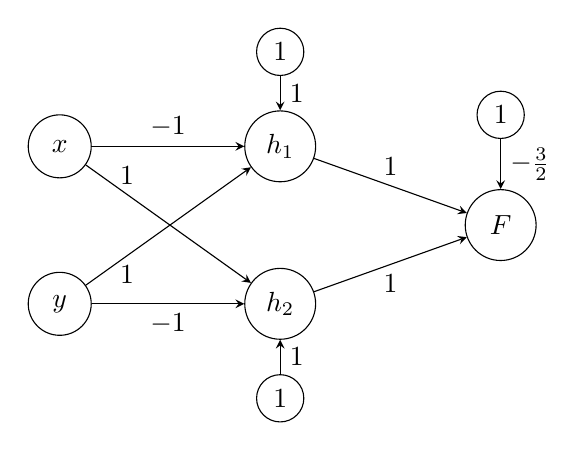
\begin{tikzpicture}[>=stealth]
  \node[draw,circle,minimum size=8mm] (x) at (0,1) {$x$};
  \node[draw,circle,minimum size=8mm] (y) at (0,-1) {$y$};
  \node[draw,circle,minimum size=9mm] (h1) at (2.8,1) {$h_1$};
  \node[draw,circle,minimum size=9mm] (h2) at (2.8,-1) {$h_2$};
  \node[draw,circle,minimum size=9mm] (f) at (5.6,0) {$F$};
  \node[draw,circle,minimum size=6mm,inner sep=0pt] (b1) at (2.8,2.2) {$1$};
  \node[draw,circle,minimum size=6mm,inner sep=0pt] (b2) at (2.8,-2.2) {$1$};
  \node[draw,circle,minimum size=6mm,inner sep=0pt] (bf) at (5.6,1.4) {$1$};

  \draw[->] (x) -- node[pos=0.5,above] {$-1$} (h1);
  \draw[->] (x) -- node[pos=0.25,above] {$1$} (h2);
  \draw[->] (y) -- node[pos=0.25,below] {$1$} (h1);
  \draw[->] (y) -- node[pos=0.5,below] {$-1$} (h2);
  \draw[->] (h1) -- node[pos=0.5,above] {$1$} (f);
  \draw[->] (h2) -- node[pos=0.5,below] {$1$} (f);
  \draw[->] (b1) -- node[pos=0.5,right] {$1$} (h1);
  \draw[->] (b2) -- node[pos=0.5,right] {$1$} (h2);
  \draw[->] (bf) -- node[pos=0.5,right] {$-\frac32$} (f);
\end{tikzpicture}
\end{center}
Les sorties sur les quatre points demandés sont respectivement $1$, $1$, $0$ et $0$.}

\item \question{Pourquoi un seul perceptron ne peut-il pas reconnaître exactement toute la bande $B$ ?}
\indication{Regarder les points $(t,-t)$ quand $t$ parcourt $\mathbb{R}$. Quelle forme prend la condition définie par un perceptron sur cette droite ?}
\reponse{Sur la droite $(x,y)=(t,-t)$, on a $(t,-t)\in B$ si et seulement si $|2t|\leq1$, soit $t\in[-1/2,1/2]$. Un perceptron seul teste une inégalité affine en $t$ sur cette droite : son ensemble de réponses $1$ est une demi-droite, toute la droite ou l'ensemble vide. Il ne peut donc pas coïncider avec cet intervalle borné.}
\end{enumerate}
}
